\section{Vlastnosti tlustovrstvých rezistorů}
-vysvětlete význam TCR, VCR, rozdíl mezi TCR a
teplotní stabilitou, výkonová zatížitelnost

\subsection{TCR}
TCR = Temperature Coefficient of Resistance (Teplotní koeficient odporu)

Všechny reálné materiály vykazují alespoň nějakou změnu odporu v závislosti na teplotě, přičemž u většiny z nich má více či méně nelineární charakter.

TCR je funkcí teploty a je definován jako sklon křivky v místě sledované teploty.

Obecně je jeho hodnota velmi malá. Je zvykem TCR vzáhnout na počáteční (okolní) teplotu a vyjádřit ho v ppm.

\begin{figure}[h]
   \begin{center}
     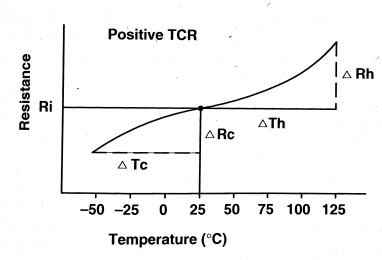
\includegraphics[scale=1]{images/TCRpos.png}
   \end{center}
   \caption{Pozitivní TCR}
\end{figure}
\begin{equation}
TCR(T) = \frac{dR(T)}{dT} \thicksim \frac{\Delta R}{\Delta T}
\end{equation}
\begin{equation}
TCR = \frac{R(T_{2})-R(T_{1})}{R(T_{1})*(T_{2}-T_{1})}*10^{-6}ppm/^{\circ}C
\end{equation}

Současně vyráběné odporové pasty mají velmi pečlivě vyvážen poměr mezi jednotlivými
složkami pasty tak, aby se TCR pokud možno co nejvíce blížilo nule - v pracovní oblasti
teplot.

Vzhledem k nelinearitě TCR je třeba si uvědomit, že se bude jeho hodnota lišit v kladných a
záporných teplotách! Proto se TCR odporových past udává (zaručuje) pouze v definovaném
teplotním rozsahu.

Dále je třeba poznamenat, že vzhledem k povaze TCR je linearizovaná hodnota
přinejlepším pouhou aproximací reálného průběhu.

TCR je u odporových past výrobci nejčastěji udáváno v následujících rozsazích:
\begin{itemize}
\item v kladných hodnotách od 25 $^{\circ}$C do 125 $^{\circ}$C
\item v záporných hodnotách od 25 $^{\circ}$C do - 55 $^{\circ}$C
\end{itemize}

Obecně by se dalo říci, že kovy vykazují pozitivní TCR. Naopak například polovodiče
negativní TCR.

U \textbf{kovů} si tuto skutečnost vysvětlujeme větší amplitudou kmitání elektronů v atomové
struktuře v důsledku dodané tepelné energie. Tím dochází ke zvýšení pravděpodobnosti
srážek s protékajícími elektrony, což se projeví jako zvýšení odporu \textbf{(pozitivní TCR)}.

U \textbf{polovodičů} naopak dodáme elektronům vázaným v krystalické struktuře materiálu
tepelnou energii, která se projeví jejich zvýšenou mobilitou. Tím se se zvyšující teplotou
stávají lepšími vodiči \textbf{(negativní TCR)}.

Pokud chceme dosáhnout co nejlepšího souběhu TCR:
\begin{itemize}
\item stejné pasty a pasty se stejným odporem na čtverec mají lepší souběh TCR
\item odpory se stejnými nebo podobnými délkami mají lepší souběh TCR
\item rezistory s blízkými nebo stejnými tloušťkami vrstev mají lepší souběh TCR
\end{itemize}

\subsection{VCR}
VCR = Voltage Coefficient of Resistance(Napěťový koeficient odporu)

Určité odporové materiály vykazují také závislost na růstu velikosti elektrického pole (V).
Rovnice vyjadřující tuto závislost je velmi podobná rovnici pro TCR.

V důsledku přítomnosti polovodičové složky materiálu v odporových pastách je VCR vždy
negativní. To znamená, že pokud V2 vzrůstá, odpor pasty klesá.


Tento efekt ze zvětšuje u past s vyššími hodnotami odporu na čtverec.

\begin{equation}
VCR = \frac{R(V_{2})-R(V_{1})}{R(V_{1})*(V_{2}-V_{1})}*10^{-6}ppm/^{\circ}C
\end{equation}

\begin{figure}[h]
   \begin{center}
     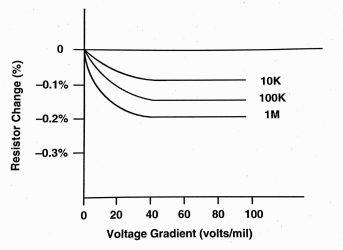
\includegraphics[scale=1]{images/VCR.png}
   \end{center}
   \caption{VCR}
\end{figure}

Z výše uvedeného vyplívá, že závislost VCR bude nepřímo úměrná také délce rezistoru.

\subsection{Teplotní stabilita}
Teplotní stabilita je u TLV rezistorů sledována z důvodu predikce změny jejich hodnoty
vzhledem k dlouhodobé tepelné zátěži (spolehlivost). Rozdíl ovšem je, zatěžujeme-li rezistor vnějším teplem (cyklovací komora) nebo jeho vlastním příkonem.

\textbf{V prvním případě} dochází k pozvolnému nárustu teploty a rovnoměrnému zvýšení teploty v celém objemu materiálu. V případě zátěže vlastním příkonem ovšem dochází k mnohem většímu lokálnímu zahřívání určitých oblastí.

Jelikož mají nízkoohmové rezistory více funkční složky (více přímých kontaktů), mají menší tendenci ke změně své hodnoty než rezistory realizované pastami s vyšším odporem na čtverec - při stejném výkonovém zatížení.

Pro většinu odporových systémů je tvar průběhu závislosti odporu na výkonovém zatížení “vzrůstající exponenciála”.

\begin{figure}[h]
   \begin{center}
     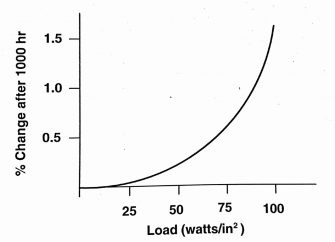
\includegraphics[scale=1]{images/Stab.png}
   \end{center}
   \caption{Teplotní stabilita}
\end{figure}

































